
% NB in Rstudio might have to go tools/options and tick `Invoke compiler via texi2dvi script'
\documentclass[a4paper]{article}
\usepackage{fancyhdr} %For headers and footers
\pagestyle{fancy} %For headers and footers
\usepackage{lastpage} %For getting page x of y
\usepackage{float} %Allows the figures to be positioned and formatted nicely
\floatstyle{boxed} %using this
\restylefloat{figure} %and this command
\usepackage{url} %Formatting of yrls
\usepackage{verbatim}
\usepackage{cite} 
\usepackage{hyperref} 
%Define all the headers and footers
\lhead{}
\chead{NCEPH Working Paper}
\rhead{}
\lfoot{Ivan C Hanigan}
\cfoot{\today}
\rfoot{\thepage\ of \pageref{LastPage}}
\usepackage{Sweave}
\begin{document}
\Sconcordance{concordance:learnR.tex:learnR.Rnw:%
1 46 1 1 21 3 1 1 2 1 0 1 1 5 0 1 9 1 2 1 0 3 1 22 0 1 2 1 3 14 0 1 2 3 %
1 1 5 5 0 1 2 14 1 1 23 5 0 1 2 25 1 1 2 23 0 1 2 4 1}

%\SweaveOpts{concordance=TRUE}
%\Sconcordance{concordance:learnR.tex:learnR.Rnw:%
1 46 1 1 21 3 1 1 2 1 0 1 1 5 0 1 9 1 2 1 0 3 1 22 0 1 2 1 3 14 0 1 2 3 %
1 1 5 5 0 1 2 14 1 1 23 5 0 1 2 25 1 1 2 23 0 1 2 4 1}

\title{Example Sweave Document}
\author{Ivan C. Hanigan$^{1}$}
\date {\today}
\maketitle
\begin{itemize}
\item [$^1$] National Centre for Epidemiology and Population Health, \\Australian National University.
\end{itemize}

\setcounter{page}{1}
\pagenumbering{roman}
\tableofcontents 
\listoftables
\listoffigures
\pagenumbering{arabic}
\setcounter{page}{1}

\section{Introduction}
This is an introduction to some resources that are useful for learning R.  
\section{The R code that produced this report}
It is important to appreciate that R is free and open source software.  This means that any code you write can be viewed and modified by others.  In some cases we need to protect our Intellectual Property and the following statement is an attempt to ascribe copyright to our work, even though it remains open source.

``I support the philosophy of Reproducible Research \cite{Peng2011}, and where possible I provide data and code in the statistical software R that will allow analyses to be reproduced.  This document is prepared automatically from the associated Sweave (RNW) file.  If you do not have access to the RNW file please contact me.''


\subsection{func}
I'll use the following packages:
\begin{Schunk}
\begin{Sinput}
> if(!require(xtable)) install.packages('xtable', repos = 'http://cran.csiro.au')
> require(xtable)
> #require(ggplot2)
> #require(ProjectTemplate)
\end{Sinput}
\end{Schunk}
\subsection{Some Code}
\begin{Schunk}
\begin{Sinput}
> x<-rnorm(100,10,5)
> y<-rnorm(100,20,15)
> fit <- lm(y~x)
> summary(fit)
\end{Sinput}
\begin{Soutput}
Call:
lm(formula = y ~ x)

Residuals:
    Min      1Q  Median      3Q     Max 
-31.482  -7.235   1.037  10.652  28.990 

Coefficients:
            Estimate Std. Error t value Pr(>|t|)    
(Intercept)  13.1925     2.8366   4.651 1.03e-05 ***
x             0.7194     0.2464   2.920  0.00434 ** 
---
Signif. codes:  0 ‘***’ 0.001 ‘**’ 0.01 ‘*’ 0.05 ‘.’ 0.1 ‘ ’ 1 

Residual standard error: 13.37 on 98 degrees of freedom
Multiple R-squared: 0.08004,	Adjusted R-squared: 0.07065 
F-statistic: 8.526 on 1 and 98 DF,  p-value: 0.004343 
\end{Soutput}
\end{Schunk}
Using the xtable package allows results to be displyed in tables and has built in support for some R objects, so summrising the linear fit above in Table ~\ref{ATable}.
% latex table generated in R 2.15.1 by xtable 1.7-0 package
% Fri Aug 31 14:12:02 2012
\begin{table}[ht]
\begin{center}
\begin{tabular}{rrrrr}
  \hline
 & Estimate & Std. Error & t value & Pr($>$$|$t$|$) \\ 
  \hline
(Intercept) & 13.1925 & 2.8366 & 4.6509 & 0.0000 \\ 
  x & 0.7194 & 0.2464 & 2.9200 & 0.0043 \\ 
   \hline
\end{tabular}
\caption{Example Table}
\label{ATable}
\end{center}
\end{table}\subsection{A Plot}
 
Plots intergrate easily, using the \LaTeX float package as can be seen in figure ~\ref{aPlot.png}.  However I like to make them as pngs and then include.

\begin{Schunk}
\begin{Soutput}
null device 
          1 
\end{Soutput}
\end{Schunk}
\begin{figure}[!h]
\centering
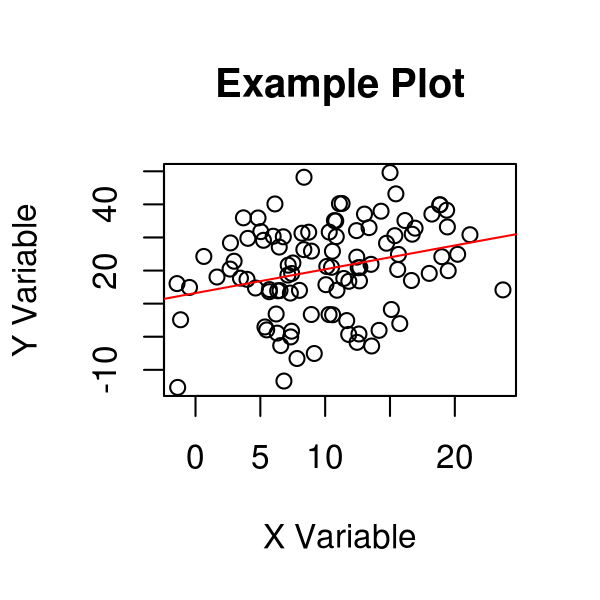
\includegraphics[width=\textwidth]{aPlot.png}
\caption{aPlot.png}
\label{fig:aPlot.png}
\end{figure}
\clearpage
\section{Remembering the points}
This blog post \url{http://www.win-vector.com/blog/2012/04/how-to-remember-point-shape-codes-in-r/} says:

I suspect I am not unique in not being able to remember how to control the point shapes in R. Part of this is a documentation problem: no package ever seems to write the shapes down. All packages just use the usual set that derives from S-Plus and was carried through base-graphics, to grid, lattice and ggplot2. The quickest way out of this is to know how to generate an example plot of the shapes quickly. We show how to do this in ggplot2. This is trivial- but you get tired of not having it immediately available.


I like it but it is not as complate as the plot shown in Figure \ref{fig:pchopts.png} from the `R for Beginners' document by Emmanuel Paradis \cite{Paradis2002}.  I also find I often get disoriented using ggplot2.

\begin{Schunk}
\begin{Soutput}
null device 
          1 
\end{Soutput}
\end{Schunk}
\begin{figure}[!h]
\centering
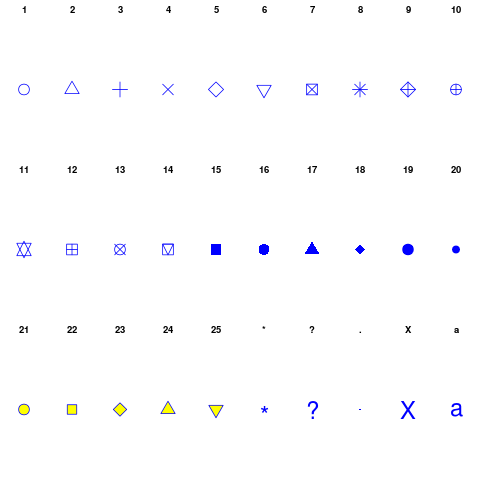
\includegraphics[width=\textwidth]{pchopts.png}
\caption{pchopts.png}
\label{fig:pchopts.png}
\end{figure}


\section{Conclusion}
In conclusion, sweave rocks.


\begin{thebibliography}{1}
\bibitem{Paradis2002}
Emmanuel Paradis.
\newblock {R for Beginners}.
\newblock 2002.

\bibitem{Peng2011}
Roger~D Peng.
\newblock {Reproducible research in computational science.}
\newblock {\em Science (New York, N.Y.)}, 334(6060):1226--7, December 2011.

\end{thebibliography}

\section{System State}
\begin{Schunk}
\begin{Sinput}
> sessionInfo()
\end{Sinput}
\begin{Soutput}
R version 2.15.1 (2012-06-22)
Platform: x86_64-pc-linux-gnu (64-bit)

locale:
 [1] LC_CTYPE=en_US.UTF-8 LC_NUMERIC=C         LC_TIME=C           
 [4] LC_COLLATE=C         LC_MONETARY=C        LC_MESSAGES=C       
 [7] LC_PAPER=C           LC_NAME=C            LC_ADDRESS=C        
[10] LC_TELEPHONE=C       LC_MEASUREMENT=C     LC_IDENTIFICATION=C 

attached base packages:
[1] stats     graphics  grDevices utils     datasets  methods   base     

other attached packages:
[1] xtable_1.7-0

loaded via a namespace (and not attached):
[1] tools_2.15.1
\end{Soutput}
\end{Schunk}




\end{document}
